\newpage
\section{Cost-benefit analyse}
Dette afsnit indeholder cost-benefit analysen, som belyser hvilke omkostninger der er forbundet med sortering af langerhanske øer. Analysen sammenligner omkostningerne forbundet med den manuelle sorteringsproces og den automatiserede metode. Formålet med analysen er, at beregne hvad stk. prisen pr. ø er ved henholdsvis den ene og den anden metode. Dette anvendes til at give en tidshorisont for hvornår en investering af den automatiserede løsning vil være tjent hjem igen. Udgangspunktet for analysen bygger på det tidsmæssige forbrug der er forbundet isolering af et batch på 400 øer fra mus. 

Fælles for begge sorteringsmetoder er, at der fortsat foretages manuel perfusion og nedbrydning og vaskning af pankreas. Nedenstående tabel opsummere hvilke basisudgifter der er forbundet ved disse processer. Timelønnen er beregnet ud fra en PhD studerendes månedsløn på 25.040 kr. REF
\begin{center}
		\begin{longtable}{ | m{6cm} | m{1.5cm} | m{1.5cm} | m{3cm}| } 
			\hline
			 &\textbf{Antal} & \textbf{Pris} & \textbf{Total}\\ 
			\hline
			 \textbf{Mus} & 6 & 60 kr & 360 kr\\ 
			\hline
			 \textbf{Timer for perfusion} & 1 & 171,62 kr & 171,62 kr\\ 
			\hline
			\textbf{Timer for nedbrydning + vask} & 1 & 171,62 kr & 171,62 kr\\ 
			\hline	
			\textbf{Total} &  &  & \textbf{703,24 kr}\\ 
			\hline
			\caption{Basis omkostninger for sorteringsproces}
			 		\end{longtable}
\end{center}
Nedenstående tabel \ref{tab:sortcost} viser, hvilke omkostninger der er forbundet med selve isoleringsprocessen af de langerhanske øer. Den halve time der bruges ved den automatiske metode er et estimat af hvad der bruges på påfyldning af beholdere og start af sorteringsproces. 
\begin{center}
		\begin{longtable}{ | m{6cm} | m{1.5cm} | m{1.5cm} | m{3cm}| } 
			\hline
			 &\textbf{Antal} & \textbf{Pris} & \textbf{Total}\\ 
			\hline
			 \textbf{Tid manuel} & 6 & 171,62 kr & 1029,73 kr\\ 
			\hline
			 \textbf{Tid automatisk} & 0,5 & 171,62 kr & 85,81 kr\\ 
			\hline
			\caption{Omkostninger ved sortering af langerhanske øer}
			\label{tab:sortcost}
			 		\end{longtable}
\end{center}
Omkostningerne ved de to sorteringsmetoder er opsummeret i tabel \ref{tab:totalcost}, herunder en samlet pris for et batch på 400 øer, og en stk. pris pr. ø for hver sorteringsmetode.
\begin{center}
		\begin{longtable}{ | m{8cm} | m{2.25cm} | m{2.25cm} | } 
			\hline
			 &\textbf{Manuelt} & \textbf{Automatisk} \\ 
			\hline
			 \textbf{Basis omkostninger} & 703,24 kr & 703,24 kr \\ 
			\hline
			 \textbf{Isoleringsomkostninger} & 1029,73 kr & 85,81 kr \\ 
			\hline
			\textbf{Total pris for sortering} & 1732,97 kr & 789,05 kr \\ 
			\hline
			\textbf{Pris pr. ø ved batch på 400 stk} & 4,33 kr & 1,97 kr \\ 
			\hline
			\caption{Opsummering af omkostninger for sorteringsprocesen for de to sorteringsmetoder}
			\label{tab:totalcost}
			 		\end{longtable}
\end{center}

Da der er forbundet omkostninger ved en investering i et system til automatisk isolering, er udgifterne til den udviklede prototype opsummeret i tabel \ref{tab:prototypecost}. I tabellen er de enkelte hardware komponenters pris noteret, samt hvad en licens til Matlab koster. Herudover er der tilføjet en profit på 400 \% af udgifterne til hardware komponenter og Matlab licens. Denne udgift dækker udgifter til support og vedligehold, produktion og-monteringsomkostninger, garanti og udvikling. Som det ses i tabellen er udgiften til den udviklede prototype beregnet til 86175 kr.
\begin{center}
		\begin{longtable}{ | m{9.5cm} | m{3.5cm} | } 
			\hline
			  & \textbf{Pris} \\ 
			\hline
			Kamera & 400 kr \\ 
			\hline
			 Ventil & 845 kr\\ 
			\hline
			Pumpe & 80 kr  \\ 
			\hline
			Arduino & 150 kr \\ 
			\hline
			Andet hardware & 210 kr \\ 
			\hline
			Beholdere + slanger & 425 kr \\ 
			\hline
			3d print & 125 kr \\ 
			\hline
			Matlab licens & 15000 kr \\
			\hline
			Profit på 400\% & 68940 kr \\	
			\hline
			\textbf{Total pris} & \textbf{86175 kr} \\		
			
			\hline
			\caption{Udgifter til automatiseret system}
			\label{tab:prototypecost}
			 		\end{longtable}
\end{center}


\newpage
Til at illustrere og sammenligne udgifterne for de to sorteringsmetoder viser figur \ref{fig:costbenefit} udgiften over tid. Figuren viser omkostningerne set over en periode på 2 år, ved at der sorteres et batch pr. uge.

\begin{figure}[H]
	\centering
	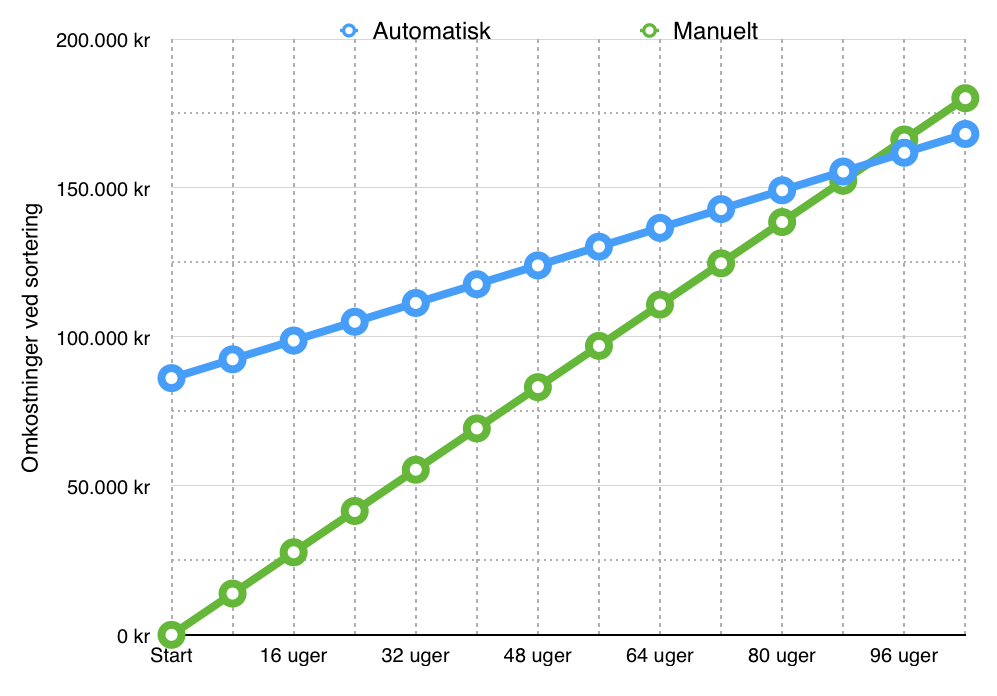
\includegraphics[width=1\textwidth]{billeder/Hovedrapport/costbenefit2.png}
	\caption{Udvikling i omkostninger }
	\label{fig:costbenefit}
\end{figure}

Af figuren ses det, at efter 92 uger overstiger omkostningerne ved den manuelle sorteringsproces de omkostninger der er ved den automatiske, og investeringen vil her være tjent hjem. 